\documentclass{article}\usepackage[]{graphicx}\usepackage[]{color}
%% maxwidth is the original width if it is less than linewidth
%% otherwise use linewidth (to make sure the graphics do not exceed the margin)
\makeatletter
\def\maxwidth{ %
  \ifdim\Gin@nat@width>\linewidth
    \linewidth
  \else
    \Gin@nat@width
  \fi
}
\makeatother

\definecolor{fgcolor}{rgb}{0.345, 0.345, 0.345}
\newcommand{\hlnum}[1]{\textcolor[rgb]{0.686,0.059,0.569}{#1}}%
\newcommand{\hlstr}[1]{\textcolor[rgb]{0.192,0.494,0.8}{#1}}%
\newcommand{\hlcom}[1]{\textcolor[rgb]{0.678,0.584,0.686}{\textit{#1}}}%
\newcommand{\hlopt}[1]{\textcolor[rgb]{0,0,0}{#1}}%
\newcommand{\hlstd}[1]{\textcolor[rgb]{0.345,0.345,0.345}{#1}}%
\newcommand{\hlkwa}[1]{\textcolor[rgb]{0.161,0.373,0.58}{\textbf{#1}}}%
\newcommand{\hlkwb}[1]{\textcolor[rgb]{0.69,0.353,0.396}{#1}}%
\newcommand{\hlkwc}[1]{\textcolor[rgb]{0.333,0.667,0.333}{#1}}%
\newcommand{\hlkwd}[1]{\textcolor[rgb]{0.737,0.353,0.396}{\textbf{#1}}}%

\usepackage{framed}
\makeatletter
\newenvironment{kframe}{%
 \def\at@end@of@kframe{}%
 \ifinner\ifhmode%
  \def\at@end@of@kframe{\end{minipage}}%
  \begin{minipage}{\columnwidth}%
 \fi\fi%
 \def\FrameCommand##1{\hskip\@totalleftmargin \hskip-\fboxsep
 \colorbox{shadecolor}{##1}\hskip-\fboxsep
     % There is no \\@totalrightmargin, so:
     \hskip-\linewidth \hskip-\@totalleftmargin \hskip\columnwidth}%
 \MakeFramed {\advance\hsize-\width
   \@totalleftmargin\z@ \linewidth\hsize
   \@setminipage}}%
 {\par\unskip\endMakeFramed%
 \at@end@of@kframe}
\makeatother

\definecolor{shadecolor}{rgb}{.97, .97, .97}
\definecolor{messagecolor}{rgb}{0, 0, 0}
\definecolor{warningcolor}{rgb}{1, 0, 1}
\definecolor{errorcolor}{rgb}{1, 0, 0}
\newenvironment{knitrout}{}{} % an empty environment to be redefined in TeX

\usepackage{alltt}
\usepackage{mathpazo}
\renewcommand{\sfdefault}{lmss}
\renewcommand{\ttdefault}{lmtt}
\usepackage[T1]{fontenc}
\usepackage[a4paper,left=2cm,right=4cm,top=2cm,bottom=2cm]{geometry}
\usepackage{setspace}
\usepackage{listings}
\usepackage{verbatim}
\usepackage{cite}

\usepackage{xspace,amsmath}
\newcommand{\um}{\ensuremath{\mu \text{m}}\xspace}
\usepackage{url}
\usepackage[authoryear]{natbib}
\newcommand{\dynamic}{(Dynamic)}
\newcommand{\static}{(Static)}
\newcommand{\hdfgroup}[1]{\texttt{#1}}
\IfFileExists{upquote.sty}{\usepackage{upquote}}{}
\begin{document}

\onehalfspacing
\title{ Exploring Ontogeny Analysis }

\author{D Hall}
\date{\today}

\maketitle










\section*{PCA}
PCA was performed on well level data and plate level data. Plate level data was obtained by taking the median of the wells on a plate. 

\begin{knitrout}
\definecolor{shadecolor}{rgb}{0.969, 0.969, 0.969}\color{fgcolor}

{\centering 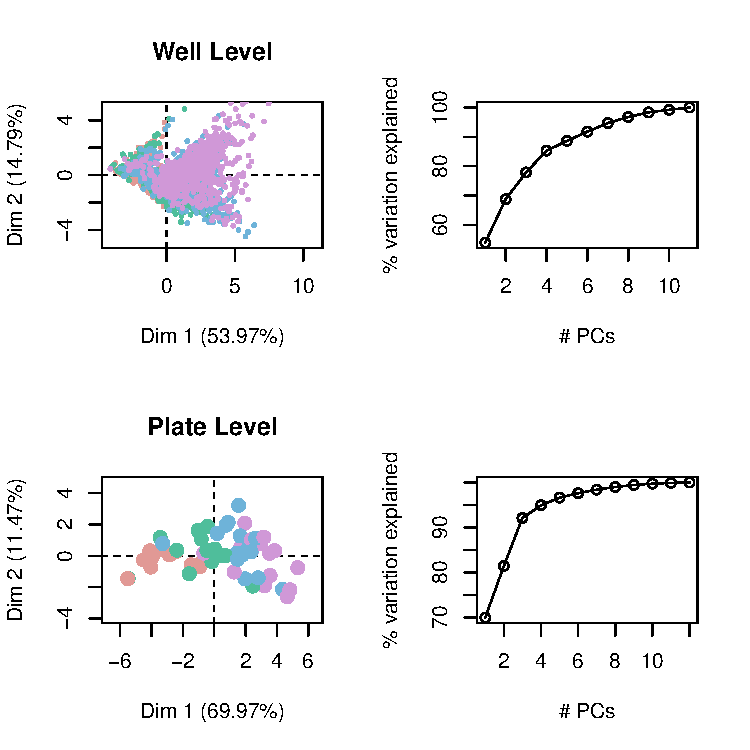
\includegraphics[width=\maxwidth]{figure/graphics-pca1-1} 

}



\end{knitrout}



\begin{knitrout}
\definecolor{shadecolor}{rgb}{0.969, 0.969, 0.969}\color{fgcolor}\begin{kframe}
\begin{verbatim}
## 
## Call:
## lm(formula = bs.pca.all$ind$coord[, 1] ~ df$DIV)
## 
## Residuals:
##     Min      1Q  Median      3Q     Max 
## -6.5694 -1.1819  0.1199  1.1037  8.3545 
## 
## Coefficients:
##             Estimate Std. Error t value Pr(>|t|)
## (Intercept) -5.33473    0.10823  -49.29   <2e-16
## df$DIV       0.64981    0.01258   51.66   <2e-16
##                
## (Intercept) ***
## df$DIV      ***
## ---
## Signif. codes:  
## 0 '***' 0.001 '**' 0.01 '*' 0.05 '.' 0.1 ' ' 1
## 
## Residual standard error: 1.769 on 2974 degrees of freedom
## Multiple R-squared:  0.473,	Adjusted R-squared:  0.4728 
## F-statistic:  2669 on 1 and 2974 DF,  p-value: < 2.2e-16
## pdf 
##   2
\end{verbatim}
\end{kframe}

{\centering 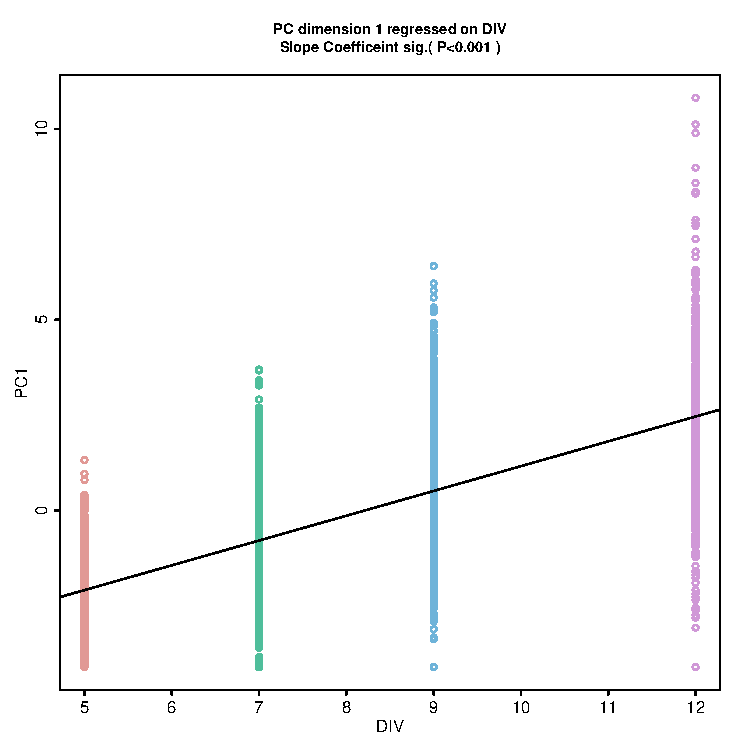
\includegraphics[width=\maxwidth]{figure/graphics-pca-ANOVA-1} 

}



\end{knitrout}





\end{document}
